\section{Grafisk bruger interface}\label{GUI_design}
\textit{Dette afsnit omhandler design, implementering og test af Graphical User Interface (GUI) til visualisering af de udførte aktiviteter. Først designes GUIen til det specifikke formål ud fra dets kravspecifikationer, hvorefter denne kan implementeres. Afslutningsvist bliver GUI testet i forhold til opstillede krav, som beskrevet i \secref{krav_GUI}.}

\subsection{Design}
GUI benyttes i dette projekt til at motivere børn til en mere aktiv hverdag. Dette gøres ud fra \secref{motivation_boern}, hvor det beskrives, at børn motiveres gennem succesoplevelser. GUI designes med henblik på at give børnene et overblik over, hvor lang tid de har udført en given aktivitet, og hvor mange point de har optjent som følge af dette. Pointene vægtes ud fra aktivitetstypen og varigheden heraf. 

Data fra algoritmerne vedrørende aktiviteterne gang og løb samt data fra gyroskopet sendes til MATLAB i form af et array med tre variable. Den første variabel i arrayet er en identifikation (ID), som angiver hvorvidt dataet kommer fra accelerometeret eller gyroskopet, som det ses på \figref{fig:GUI}. IDet for accelerometeret er 2, mens IDet for gyroskopet er 3.\\
Hvis MATLAB registrerer accelerometerets ID, benyttes peakværdien på anden plads i arrayet. Denne værdi gør, at gang og løb kan adskilles og informerer dermed om, hvilken aktivitet tidsvariablen skal lægges til. På tredje plads findes en tidsenhed, som er resultat af varighed siden sidst detekterede peak. Er peakværdien mellem 100 og 1100 skal varigheden lægges i tidsvariablen for gang, og er den lig med eller over 1100 skal den lægges over i tidsvariablen for løb.\\
Registreres gyroskopets ID, påbegyndes databehandlingen heraf i MATLAB, som er beskrevet i \secref{sec:algocykel}. Giver resultatet af denne databehandling en værdi over 70\% overføres fire sekunder til tidsvariablen for cykling til GUIen.\\ 
På første plads i gyroskopets dataarray findes 3 tallet, der er ID for gyroskop data. Anden plads indeholder gyroskopdata. På den tredje plads i arrayet er tallet 4 repræsenteret, som ikke bruges i nogen beregninger. Denne er til for at mikrokontrollerens array for alle tre aktiviteter er lige lange. 

Hver aktivitet belønnes forskelligt, da cykling og løb har højere intensitetsniveau end gang, hvormed pulsen stiger for disse aktiviteter, og dermed også det fysiologiske udbytte. Derfor omregnes tiden til point ved at multiplicere tiden for løb med 3, for cykling med 2 og for gang med 1.\\ 
Pointene visualiseres i GUI ud for den enkelte aktivitet, hvorved barnet kan se, hvor mange point vedkommende har opnået ved udførsel af hver aktivitet igennem en hel dag. For at give barnet bedre visualisering af udført aktivitet over en periode summeres pointene for hver dag og plottes i en graf. Pointene vises grafisk som en søjle med individuelle farver for hver aktivitet, hvormed barnet yderligere kan se hvor stor en del, hver aktivitet har udgjort af dagens totale point.  
\begin{figure}[H]
	\centering
	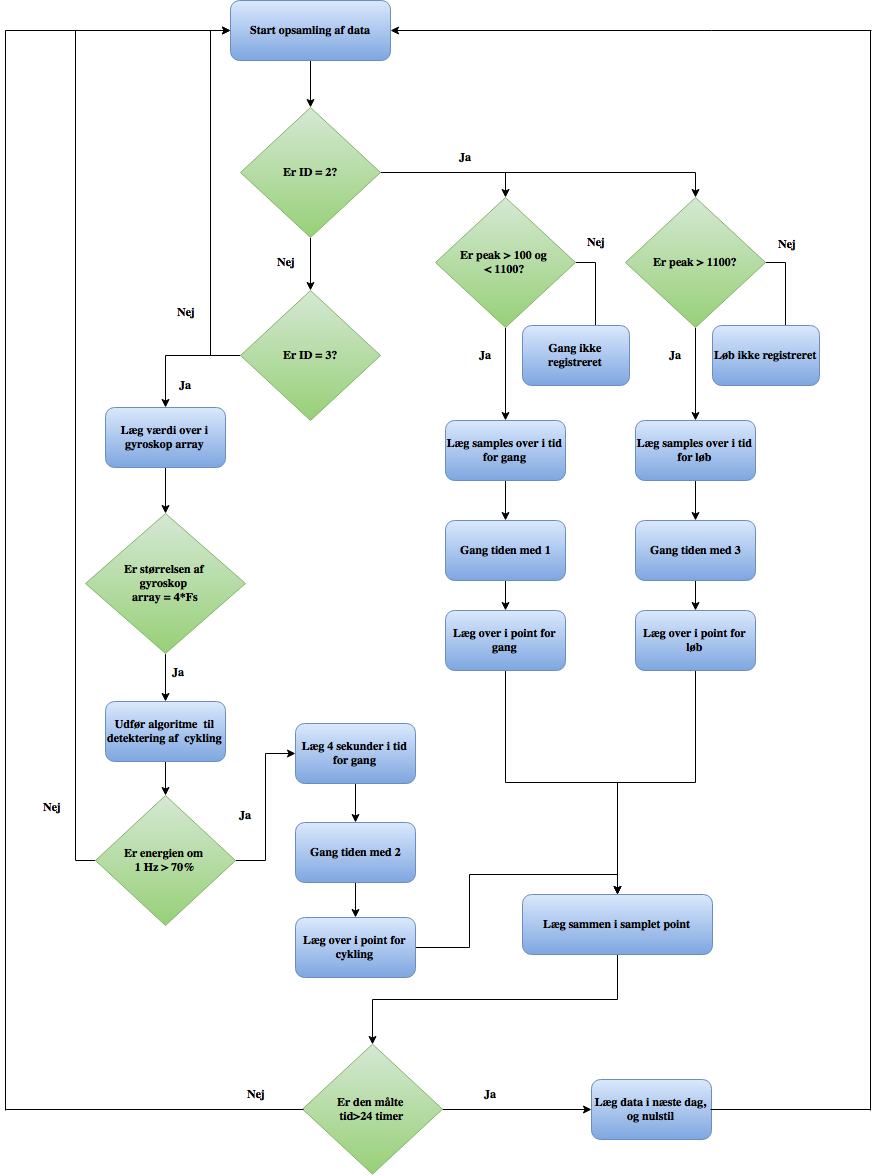
\includegraphics[scale=0.4]{figures/cDesign/pseudo_GUI.png}
	\caption{På figuren ses et flowchart, der gennemgår hvorledes resultaterne fra de forskellige algoritmer behandles af GUI.}
	\label{fig:GUI}
\end{figure}

\subsection{Implementering}
GUI implementeres ved at skabe en figur i MATLAB hvori brugerens tid og point printes i en tabel for hver aktivitet samt total for alle dagens aktiviteter. Hertil plottes et søjlediagram over brugerens point for dagen, plottet i tre forskellige farver alt efter aktiviteten. Dette plottes for tre dages aktivitet, således at brugeren kan følge sin progression. 
%GUI implementeres ved at anvende MATLABs funktion Graphical User Interface Design Environment (GUIDE). GUIDE er en funktion, der gør det muligt at lave en specifik brugerflade med indbyggede funktioner.

Programmet starter idet der trykkes 'Run' i MATLAB, hvorved indhentning af data fra mikrokontrolleren begynder. Programmet benytter ved hjælp af if løkker, den første værdi i arrays på 3, til at adskille accelerometerdata og gyroskopdata. \\
Er den første værdi 2 i det indhentede array, registreres mikrokontrollerens data som værende accelerometerdata. Den anden værdi i arrayet er en repræsentation af, hvor mange samples der er mellem hvert peak. Denne skal omregnes til minutter og lægges over i tidsvariablen for den pågældende aktivitet. Omregning udføres som ses i \eqref{eq:tidsvariabel}. Den tredje værdi angiver peakværdien, hvilken indikerer om aktiviteten er gang eller løb. \\
Er den første værdi i arrayet 3, registreres mikrokontrollerens data som værende gyroskopdata. Den anden værdi i arrayet lægges derefter over i et nyt array der behandles som beskrevet i \secref{sec:algocykel}. En tidsvariabel på fire sekunder lægges derefter over i cykling, hvis databehandlingen viser at energien omkring den maksimale peak summeret fra $\pm$1~Hz er over 70\%. Den tredje værdi i arrayet er et 4-tal som har til funktion, at sørge for at længden af arrayet et den samme som for accelerometerdataet, hvorfor denne værdi ikke benyttes til databehandling.   
%Der indsættes en grøn toggle button med teksten START, og når der trykkes på knappen starter programmet. Herefter bliver knappen rød, og teksten ændres til STOP. Når programmet starter indhentes data fra mikrokontrolleren. \\
%Er den første værdi 2, registreres mikrokontrollerens array som værende data fra accelerometeret. Den anden værdi i arrayet er en repræsentation af, hvor mange samples der er mellem hvert peak. Denne skal omregnes til minutter og lægges over i tidsvariablen for den pågældende aktivitet. Omregning udføres som ses i \eqref{eq:tidsvariabel}. Den tredje værdi videreføres til løkker, hvori der tjekkes for, om peakværdien indikerer aktiviteten gang eller løb. \\
%Er den første værdi 3, registreres mikrokontrollerens array som værende data fra gyroskopet. Den anden værdi i arrayet lægges derefter over i et nyt array på 4*Fs og behandles som beskrevet i \secref{sec:algocykel}. En tidsvariabel på fire sekunder lægges derfor over i cykling, hvis databehandlingen viser at energien omkring maks peak summeret med værdien fra $\pm$1~Hz er over 70\%. 
\begin{equation}
Tidsvariabel = \frac{Samples}{Samplingsfrekvens} \cdot 0,016667
\label{eq:tidsvariabel}
\end{equation}

Tidsvariablen benyttes til at udregne point for aktiviteterne. Dette gøres ved at multiplicere med de tidligere nævnte værdier opnået som følge af aktivitetstypen. Dette ses i \eqref{eq:pointvariabel}. 
\begin{equation}
Pointvariabel = Tidsvariabel \cdot Aktivitetspoint
\label{eq:pointvariabel}
\end{equation}

Tidsvariablen og pointvariablen for de enkelte aktiviteter lægges over i forskellige static text felter. Disse tilhører henholdsvis point og tid for de tre forskellige aktivitetstyper. Ydermere er der to forskellige static text, hvor der i den ene samles tidsvariablerne for hele dagen, og i den anden samles point opnået gennem hele dagen. \\
Der implementeres et søjlediagram med faste axis værdier, hvor data plottes. I denne samles point fra gang, løb og cykling, som plottes oven på hinanden med forskellige farver. Dette gør det muligt at se hvilke aktiviteter der er udført, og hvor mange point de summeret giver for en dag. \\
I programmet er der aktiveret en timer, hvilket gør det muligt at skifte til en ny dag efter 24 timer. Ved begyndelse på en ny dag nulstilles alle variabler, og der plottes i den næste dag.\\ 
Afslutningsvist kan programmet stoppes ved at der trykkes 'Q' på tastaturet. Herved stoppes dataindhentningen og optællingen af aktivitetstid samt tilhørende point, hvorfor figuren fryses og derefter kan lukkes. 

\subsection{Test}
Testen udføres på baggrund af de opstillede krav og tilhørende tilladte afvigelser opstillet i \secref{krav_GUI}, som beskriver, at GUIen skal:
\begin{itemize}
	\item Kunne visualisere tidsforbruget og point opnået ved henholdsvis gang, løb og cykling.  
\end{itemize}

%%%%%%%%%%%%%%%%%%%%%%%%%%%%%%%%%%%%%%%%%%%%%%%%%% GAMMELT %%%%%%%%%%%%%%%%%%%%%%%%%%%%%%%%%%%%%%%%%%%%%%%%%%%%
Testen udføres ved at indsende kendte værdier, hvoraf hver aktivitet kan testes individuelt i forhold til multiplikation som følge af aktivitetstype.
Igennem testen indsendes et datasæt med simuleret input fra algoritmen, som skal trigge de forskellige aktiviteter. For gang indsendes [2 512 1050], for løb indsendes [2 512 1150] og for cykling indsendes [3 (35$\cdot$sin(2$\pi$)$\cdot$0,5$\cdot$(2t))+60) 4]. De forskellige aktiviteter simuleres 60$\cdot$6 gange, hvormed et simuleret signal på 6 minutter opnås.

Resultatet af GUIs design gør at forskellige aktivitetsformer bidrager til en forskellig mængde point. Ligeledes er varigheden og intensiteten  af aktiviteten afgørende for mængden af opnåede point, på baggrund af deres multiplikationsfaktor, hvilket kan ses i \eqref{eq:pointvariabel}
\begin{table}[H]
	\centering
	\begin{tabular}{ccc}
		\hline
		\rowcolor[HTML]{C0C0C0} 
		Aktivitet 	& Forventet antal point & Optalt antal point \\ \hline
		Gang 	&  6 & 6  \\ \hline
		Løb 	& 18 & 18 \\ \hline
		Cykling & 12 & 12 \\ \hline
	\end{tabular}
	\caption{I tabellen ses sammenhængen mellem forventede antal point og optalt antal point, som resultat af den indsendte simulerede data.}
	\label{test:GUI}
\end{table}\vspace{-.5cm}
På baggrund af testen, konkluderes det at GUIen fungerer efter hensigten. De forventede antal point og optalt antal point var nøjagtig det samme. Disse optjente point visualiseres i et søjlediagram som beskrevet i design. Varigheden af hver aktivitet visualiseres som en værdi, der summeres op hver gang et aktivitetsresultat bliver behandlet. Resultatet af at indsende det simulerede data afspejlet i GUI kan ses på \figref{fig:GUI2}\fxnote{lav ny figur!!!}.

\begin{figure}[H]
	\centering
	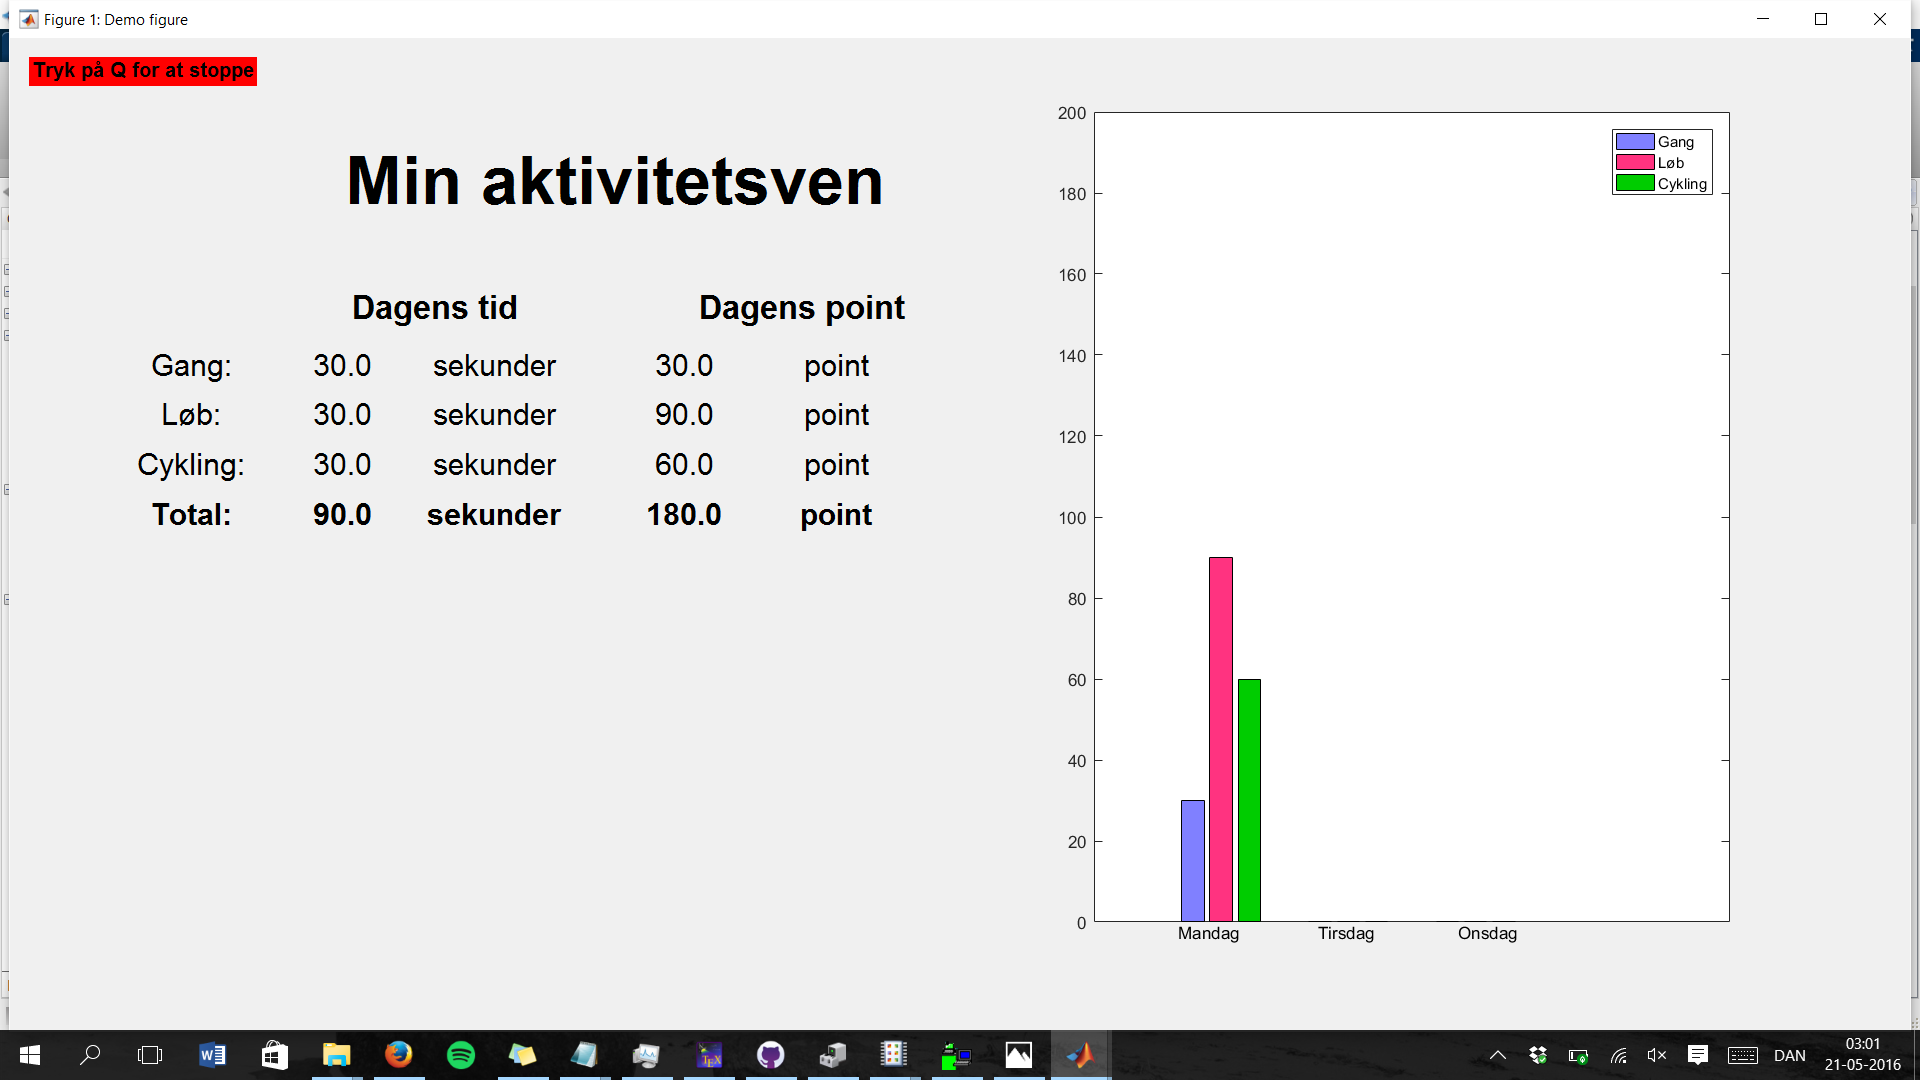
\includegraphics[scale=0.7]{figures/cDesign/test_GUI.png}
	\caption{På figuren ses et udklip af GUI hvor udførslen af aktiviteterne gang, løb og cykling visualiseres. Aktiviteternes samlede antal point og udført varighed ses på figuren.}
	\label{fig:GUI2}
\end{figure}

Efterfulgt af design, implementering og test af GUI, kan det konkluderes at denne opfylder kravene heraf. GUI er i stand til at visualisere tidsforbruget samt antal point opnået, for alle aktiviteterne. GUI opdaterede kontinuert i testen hver gang et nyt input blev indsendt, hvoraf kravet vedrørende opdatering af GUI mindst hvert femtende minut, ligeledes er opfyldt.